\documentclass[fleqn,10pt]{wlscirep}
\usepackage[utf8]{inputenc}
\usepackage[T1]{fontenc}

\usepackage[demo]{graphicx}
%\usepackage{caption}
\usepackage{subcaption}

\title{From Surface To Depth -- thinking the next step of the inverse problem of electrocardiography}

% \author[1,*]{Alice Author}
% \author[2]{Bob Author}
% \author[1,2,+]{Christine Author}
% \author[2,+]{Derek Author}
% \affil[1]{Affiliation, department, city, postcode, country}
% \affil[2]{Affiliation, department, city, postcode, country}
% \affil[*]{corresponding.author@email.example}
% \affil[+]{these authors contributed equally to this work}

% For quotes
\newenvironment{itquote}
{\begin{quote}\itshape}
{\end{quote}}

\author[1,2]{Roland Stenger}
\author[1,3] {Baltasar R\"uchardt}
\author[1,3,4] {Stefan Luther}
\author[1,2,3,*] {Ulrich Parlitz}

\affil[1]{Max Planck Institute for Dynamics and Self-Organization, Am Fassberg 17, 37077 G\"ottingen, Germany}
\affil[2]{Institute for the Dynamics of Complex Systems, University of G\"ottingen, 
	      Friedrich-Hund-Platz 1, 37077 G\"ottingen, Germany}
\affil[3]{German Center for Cardiovascular Research (DZHK), partner site G\"ottingen, Robert-Koch-Str. 42a, 37075 G\"ottingen, Germany}
\affil[4]{Institute of Pharmacology and Toxicology, University Medical Center G\"ottingen,   Robert-Koch-Str. 40, 37075, G\"ottingen, Germany}

\affil[*]{ulrich.parlitz@ds.mpg.de}


%\keywords{Keyword1, Keyword2, Keyword3}

\begin{abstract}
\textcolor{red}{Example Abstract. Abstract must not include subheadings or citations. Example Abstract. Abstract must not include subheadings or citations. Example Abstract. Abstract must not include subheadings or citations. Example Abstract. Abstract must not include subheadings or citations. Example Abstract. Abstract must not include subheadings or citations. Example Abstract. Abstract must not include subheadings or citations. Example Abstract. Abstract must not include subheadings or citations. Example Abstract. Abstract must not include subheadings or citations.}
\end{abstract}
\begin{document}
\flushbottom
\maketitle
\thispagestyle{empty}
%\noindent Please note: Abbreviations should be introduced at the first mention in the main text – no abbreviations lists. Suggested structure of main text (not enforced) is provided below.

\section{Introduction}
% 


% The Introduction section, of referenced text\cite{Figueredo:2009dg} expands on the background of the work (some overlap with the Abstract is acceptable). The introduction should not include subheadings.

%The inverse problem of electrocardiography (inverse ECG) describes the attempt to reconstruct the electrical signal on the heart surface based on electrocardiogram (ECG) measurements. This tasked is broadly studies \cite{many citations} and gets even more attention in recent years. However the ECG measurements are based on potential measurements and as a) potential is expected to be continuous and b) the heart is an active medium, the potential can be reconstructed to the heart surface but how to deal with the interactive heart medium remains unclear. Therefore we focus on this second part 'from the surface into the muscle' which is challenging because an appropriate model for (electrical) dynamics of the heart is an excitable medium. In this it is not clear per se, what information about the state in the depth can be obtained from the state on the surface.

\textcolor{red}{In this article we examine how deep we can 'look' into the heart based on surface information on 2 different sides on a cube, where the dynamics have been learned by neuronal networks.}


%-> Ecg
%-> loss of information
%-> inverse ecg
%-> reconstruction techniques give surface activity
%-> from surface to inside muscle: excitable medium
%-> question: How can the 'inverse excitable medium' problem be tackled?
%(-> literature?)
%-> Machine learning via neuronal networks
\section{Methods}\label{sec:methods}
%Topical subheadings are allowed. Authors must ensure that their Methods section includes adequate experimental and characterization data necessary for others in the field to reproduce their work.

In this section we first introduce in section \ref{sec:exmedia} the mathematical model for simulating excitable media. Furthermore, the individual steps which are necessary for generating both regimes, are explained. 
Following, in section \ref{sec:models} we introduce the machine learning model for facing the task: reconstructing excitations under the surface of the cube.

\subsection{Simulation of excitable media}\label{sec:exmedia}
\textcolor{red}{Einleitende Worte...}
\subsubsection*{Barkley model}
There are various models to describe the heart dynamic with differential equations in terms of voltage current. Since the experiments goal is to reconstruct hidden regions under the surface qualitatively, the model for excitable media does not have to provide a realistic approximation of the heart's electrical activity in terms of current voltage. The Barkley model is a model for excitable media and is a system of two coupled differential equations with the variables $u$ and $v$, which build a reaction diffusion system. It was proposed by Barkley et al. in 1990 \cite{barkley_spiral_wave_1990}.

The model is given by the equations

\begin{align}
    \frac{\partial u}{\partial t}&=D\cdot \nabla^2u+\frac{1}{\varepsilon}(1-u)\left(u-\frac{v+b}{a}\right),\notag\\
    \frac{\partial v}{\partial t}&=u^{\alpha}-v,\notag\\
    \label{eq:barkley}
\end{align}

where $u$ is a fast variable, while the variable $v$ is slower and inhibiting \cite{berg_synchronization_2011}.
The parameter $a$, $b$ and $\epsilon$ are positive constants. A bigger value for $a$ increased the excitation duration while an increasing fraction between $b$ and $a$, $\frac{b}{a}$, results in a larger excitability threshold \cite{Barkley_2008}. 

% HYPERPARAMETER
    % - Genaue Werte für a,b, epsilon
    % - Simulationsmethode
%In this work the value for $\alpha$ is set to 3, which can cause chaotic behavior. Here, two sets of parameters are tested, where $a$, $b$ and $\epsilon$ are varied, as well as the starting values for $u$ and $v$. One regime is periodical, while the other shows chaotic behaviour. Both are simulated with 

\subsubsection*{Characteristic variables}
To have a more intuitive understanding about temporal and spatial sizes, the following characteristic variables are introduced:

\begin{itemize}
    \item Time $T_c$: The characteristic time $T_c$ is defined by average period length, which is estimated by identifying peaks within the time series of individual voxels from simulations of regime A. As described in section \ref{cap:datarecording}, a part of the simulated data consists of 2048 recordings from simulations which last, after an initial phase, over a time span of 512 time steps, which are recorded in intervals of 16 time steps. When two peaks are identified within the time series of a voxel, the gap between them is then saved as a single period length. These lengths, calculated from each voxel on each simulation are used to compute the mean period length, which is considered as characteristic time.
    \item Length $\lambda_c$: An other part of the simulation data, as described in section \ref{cap:datarecording}, consists of 2048 recordings from simulations at a certain time step, which include the data till a depth of 32 discrete spatial units. Therefore, the data can be represented by a tensor with the dimensionality of (32,120,120). 
    From this data, the values of the voxels along vectors in x- and y-direction along the axes with length 120 are used. From each individual simulation, 120*32 vectors of length 120 follow, which consist of the respective $u$-values of the simulations. In these series, the positions of the peaks at which $u$ reaches a local maximum are determined, and then the distance to the next peak is calculated. A histogram of the collection of all distances from each simulation is shown in figure \ref{fig:dist_characteristic_length}. The first maximum of this histogram is regarded as characteristic length. The error of this value is estimated with $0.5\Delta s$.
\end{itemize}

\begin{figure}[ht]
    \center
    \includegraphics[width=0.8\textwidth]{figures/dist_characteristic_length}
	\caption{Histogram from the distances between two peaks of the $u$-value, which are recorded along vectors in $x$- and $y$-direction on the simulated cube geometry till a depth of 32.}
	\label{fig:dist_characteristic_length}
\end{figure}

The resulting values for $\lambda_c$ and $T_c$ are shown in table \ref{tab:characteristic}. Since in both regimes the discretization of time and space ($\Delta t$ and $\Delta s$) are used, the characteristic variables, scaled with the discretizations are used in the further process. However, due to the chaotic behaviour of regime B, no spiral waves are formed on which such a determination of the characteristic variables would be possible.

\begin{table}[h]
    \centering
    \caption{Characteristic variables for the Barkley regime A.}
    \begin{tabular}{|c|c|}
    \hline
    $\lambda_c$ & $(16.2\pm0.5)\cdot\Delta s$ \\ 
    \hline
    $T_c$ & $(74.93\pm5.45)\cdot\Delta t$ \\
    \hline
    \end{tabular}
    \label{tab:characteristic}
\end{table}

From the two variables $\lambda_c$ and $T_c$, a characteristic velocity can be extracted, which results to 

\begin{align}
    v_c=\frac{\lambda_c}{T_c}=(0.22\pm0.02)\frac{\Delta s}{\Delta t}.
\end{align}

A wave-front which propagates along the normal of the surface in a depth of $\lambda_c$, needs approximately 74.93 discrete time steps to be recognisable at the surface, since it is estimated to propagate with a speed of $v_c$.
\subsubsection*{Starting conditions}
In the following, the procedure of generating unique starting conditions in each new simulation is explained, where the characteristic properties for regime A (periodic dynamics) and regime B (chaotic dynamics) remain the same.

\subsubsection{Regime A, periodic spiral waves}
To initiate spiral waves, the cube in which the simulation takes place, is firstly divided into 8 sub cubes of equal size. The following procedure is the same for two of the 8 sub cubes. In the 6 remaining, the values for $u$ and $v$ are set to 0 at every voxel.

First, the sub cube is \textit{filled} up till a random height (as shown in the left graphic of figure \ref{fig:u_evolution}), where the $u$-value is set to 1.0 at every voxel inside. The same procedure takes place for the $v$-value, but rotated by 90 degree, whose values are set to 0.5. Visualized is this procedure in the left figures of \ref{fig:u_evolution} and \ref{fig:v_evolution}. In the next step, this structure is rotated around all three axes randomly, but remains the same for $u$- and $v$-value for one sub cube. As third step, the two sub cubes on which this procedure was performed, are placed diagonally to each other, so that these, with the remaining 6 sub cubes, form the shape of the original cube. This is the initial situation with which the simulation starts.The height till which the sub cubes gets \textit{filled} is random, as well as the rotations. The left plot in figure \ref{fig:timelines} shows an example of a single voxel within the simulation whose $u$-value is plotted against the time. The periodicity behaviour (after an initial phase) can be seen here.

\begin{figure}[ht]
    \center
    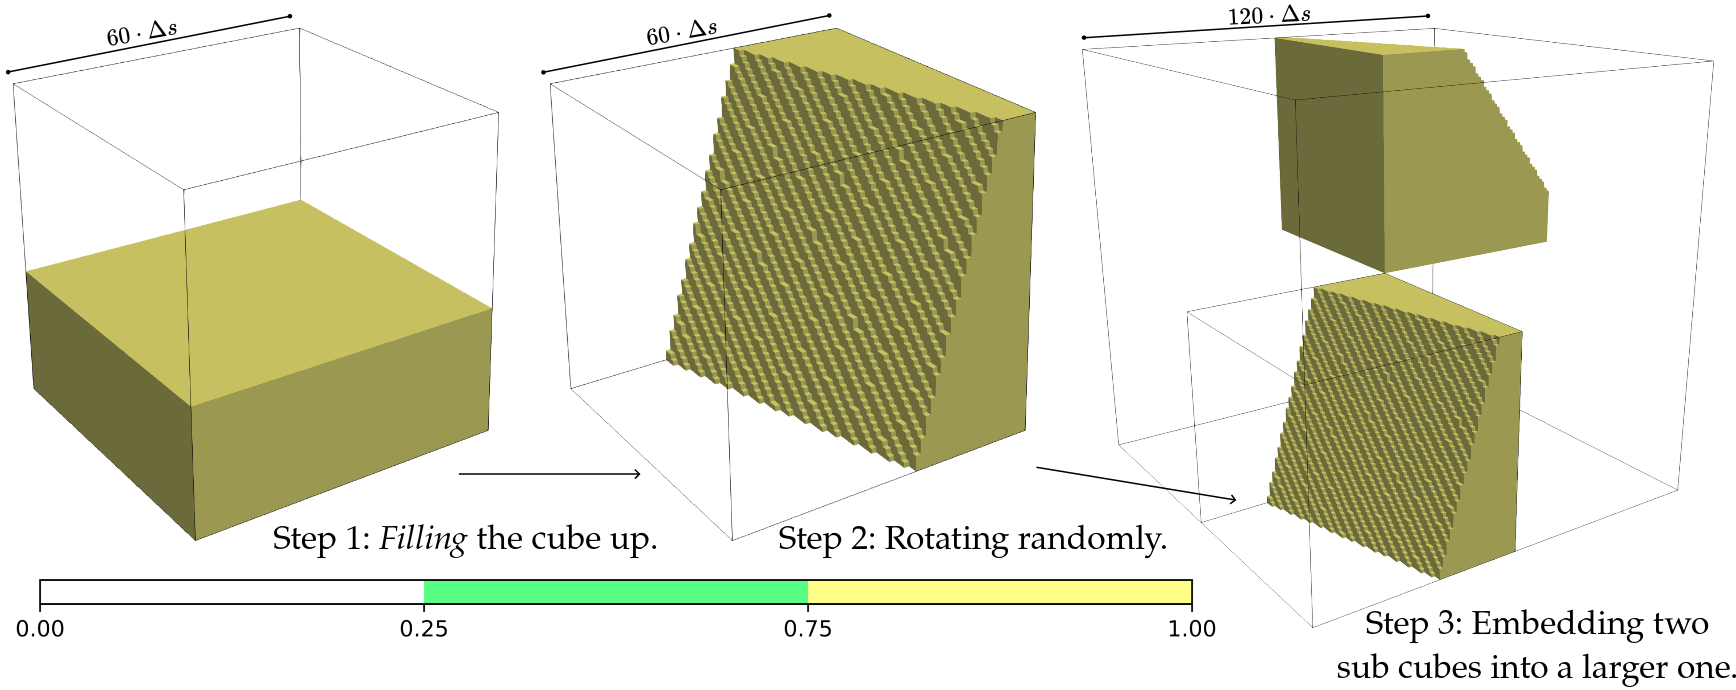
\includegraphics[width=0.7\textwidth]{figures/u_evolution.png}
	\caption{Procedure of generating starting conditions for the $u$- and $v$-value. Visualized is the $u$-value at each step within the procedure.}
	\label{fig:u_evolution}
\end{figure}

\begin{figure}[h]
    \center
    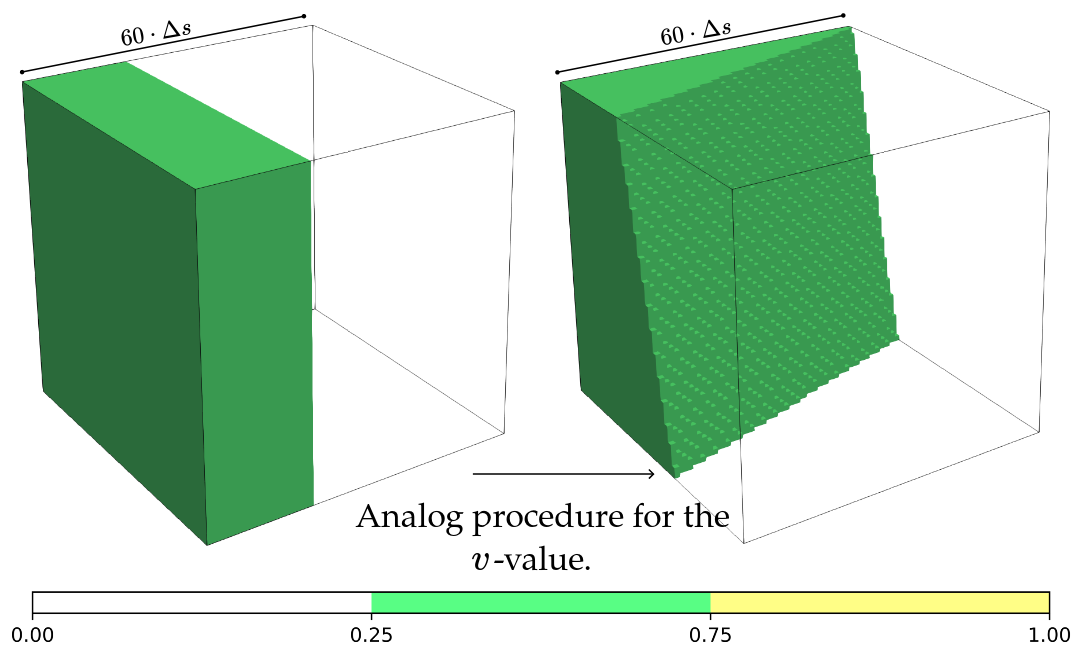
\includegraphics[width=0.5\textwidth]{figures/v_evolution.png}
	\caption{Procedure of generating starting conditions for the $u$- and $v$-value. Visualized is the $v$-value at the first two steps within the procedure.}
	\label{fig:v_evolution}
\end{figure}


\subsubsection{Regime B, chaos}
To generate chaos, not only the Barkley parameter $a$, $b$, $\epsilon$ and $\alpha$ are critical, but also the starting conditions. The cube is firstly divided into equilateral cubes of length $6\cdot\Delta s$ in each dimension, where every voxel in a single sub cube has the same $u$- and $v$-value of the Barkley model. The values for $u$ are randomly chosen between 0 and 1 from an equal distribution. If the value exceeds 0.4 in a sub cube, $v$ is set to 0 in the same sub cube. If it is not the case, $v$ is set to 1.0. The right plot in figure \ref{fig:timelines} shows an example of a single voxel within the simulation whose $u$-value is plotted against the time. It can be seen that there is no periodicity as in the left graphic.

\begin{figure}[h]
    \center
    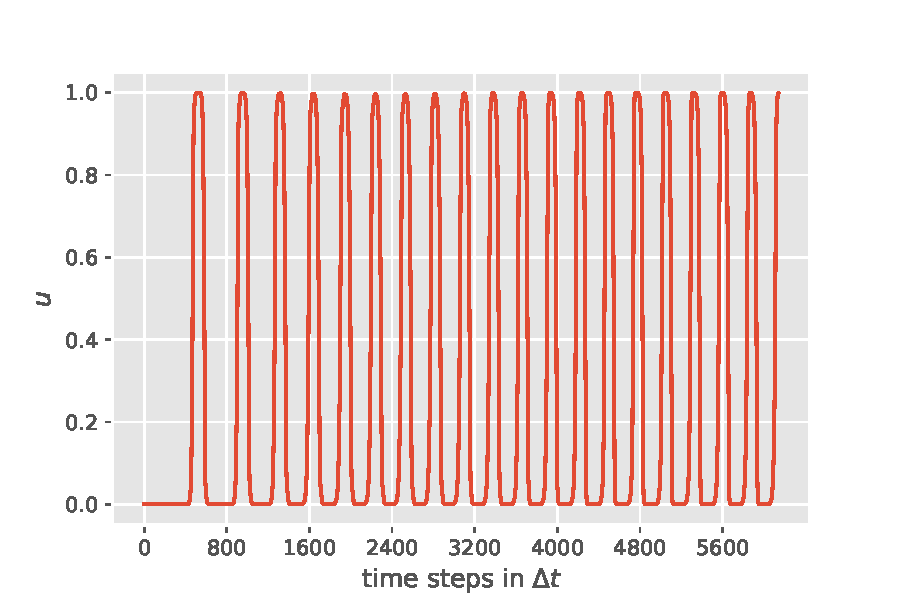
\includegraphics[width=0.45\textwidth]{figures/timeline_periodic.pdf} 
    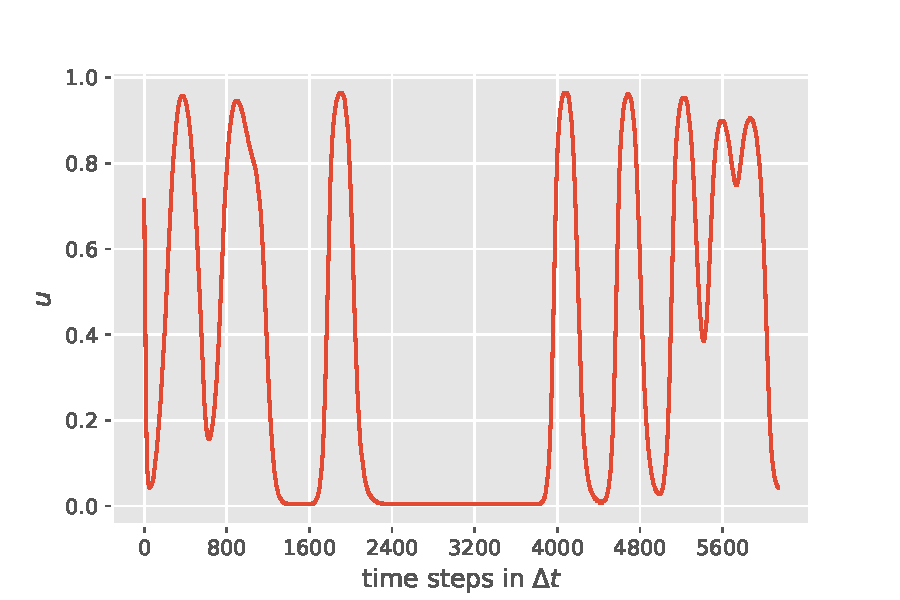
\includegraphics[width=0.45\textwidth]{figures/timeline_chaotic.pdf} \\
    \caption{Time development of the $u$-value of a single voxel from a simulation in the (left) periodic regime A and (right) the chaotic regime B.}
 \label{fig:timelines}
\end{figure}

%\subsubsection*{Barkley model}


%More details about the regimes are in section \ref{cap:regimes}, where the values for $a$, $b$ and $\epsilon$ are listed in table \ref{tab:params_regimes}.

\subsection{Machine learning methods}\label{sec:model}
% Why is it seq2seq?
In this section, we introduce the spatio temporal long-short-term-memory (ST-LSTM) \cite{stlstm}, a special kind of recurrent neural network (RNN), which is applied to perform the reconstruction task as defined in section [XXX], a kind of sequence-to-sequence (seq2seq) problem.

\subsubsection{Recurrent neural networks}
Recurrent neural networks (RNNs) are prominent when it comes to seq2seq problems, where the network is trained to convert a sequence to another sequence. A famous task in this domain is machine translation where a sequence of words in one language is transformed to another sequence of words of a different language. Other important tasks are for example speech-recognition where an encoded voice recording has to be converted into a sequence of words, or next-frame-prediction, a task to predict the future frames of a video. In each example, recurrent networks were considered as state-of-the-art, at least for a while \cite{seq2seq_example1} \cite{seq2seq_example2} \cite{seq2seq_example3}.

%Intro (what problems for example)
A recurrent neural network is a form of neural network which is, in combination with an iterative update loop of its internal state (memory), able to process through an input sequence with varying length. With every iteration, an internal state, the \textit{hidden state}, which has a fixed dimensionality, is evolving to be dependent on every previous time step. The \textit{hidden state} can be calculated regardless of the length of the input sequence and provides a representation of the sequence.

A characteristic that is generally seen with seq2seq problems is that both the input sequence and the output sequence are of variable length. For example, a translation model has to be able to take a sequence with varying length of words to output a translation as a sequence with a varying length as well. Furthermore, a strong translation model should be able to translate single words as well as a long sequences of hundreds of words. In this work, the problem of the numerical experiment also faces the characteristic of a seq2seq problem, where a recurrent neural network is used as well.

%\begin{figure}[ht]
%    \center
%    \includegraphics[width=0.50\textwidth]{figures/rnn_schamtic}
%	\caption{Visualization of the calculations within an Elman network.}
%	\label{fig:rnn_schematic}
%\end{figure}

% Exact definition
\subsubsection{Long short-term memory (LSTM)}

The following equations describe the computations within the probably most famous recurrent neural network, the Long short-term memory (LSTM). Given a sequence of inputs $(x_1,x_2,...,x_T)$, the LSTM not only evolves a hidden state $h_t$, but also a cell state $C_t$ such as 

\begin{align}
    g_t&=\tanh\left(\textbf{W}_{cx}\cdot x_t + \textbf{W}_{ch}\cdot h_{t} + b_g\right), \notag\\
    i_t&=\sigma\left(\textbf{W}_{ix}\cdot x_t + \textbf{W}_{ih}\cdot h_{t} + b_i\right), \notag\\
    f_t&=\sigma\left(\textbf{W}_{fx}\cdot x_t + \textbf{W}_{fh}\cdot h_{t} + b_f\right), \notag\\
    o_t&=\sigma\left(\textbf{W}_{ox}\cdot x_t + \textbf{W}_{oh}\cdot h_{t} + b_o\right), \notag\\
    C_{t+1}&=f_t\circ C_{t}+i_t\circ g_t, \notag\\
    h_{t+1}&=o_t\circ\tanh(C_t),\notag\\
    \label{eq:lstm}
\end{align}

Furthermore, it provides an output sequence $(o_0,o_1,...,.o_T)$ of the same length as the input sequence. The function $\tanh$ is the hyperbolic tangent, and $\sigma$ is the logistic function. The symbol $\circ$ denotes the Hadamard product, also known as pointwise multiplication.\\% The computations within a LSTM are graphically shown in figure \ref{fig:LSTM}. \\

The neural network to face the seq2seq problem in this experiment is based on the LSTM design with three adjustments, that are made address specific problems in this special task, which are described in the following:

%\begin{itemize}
%    \item Stacking LSTM layers: A method for stacking RNNs is taking the output sequence ($y_1$, ..., $y_T$) or the sequence of hidden states ($h_1$, ..., $h_T$) as input for a new RNN. Although it is not theoretically clear why stacked RNNs perform in certain tasks better than single-layer RNNs, in practice they provide a higher learning capacity \cite[p.51]{goldberg_primer_2015}.
%    \item Convolutional operations instead of linear feed-forward layer
%    \item Spatio-temporal LSTM: Evolving another state $M$ which \textit{flows} through space and not exclusively through time. In a stacked convolutional LSTM, spatial correlations and temporal dynamics are not equally processed\cite{prednet}, however, these two aspects might be equally important and should be considered equally significant in a machine learning model for spatio-temporal data.
%\end{itemize}

To address the problem mentioned in the last point, Y. Wang et al. introduce in their paper \textit{PredRNN:Recurrent Neural Networks for Predictive Learning using Spatio-temporal LSTMs}\cite{prednet} a variation of the LSTM and its integration into a stacked recurrent neural network. They do not define how to measure the equality in processing the two aspects (spatial correlations and temporal dynamics) but they formulate it as follows:

\begin{itquote}
[...] spatial representations are encoded layer by layer, with hidden states being delivered from bottom to top. However, the memory cells that belong to these [...] layers are mutually independent and updated merely in time domain. Under these circumstances, the bottom layer would totally ignore what had been memorized by the top layer at the previous time step.
\end{itquote}

\begin{figure}
\centering
\begin{subfigure}{.5\textwidth}
  \centering
  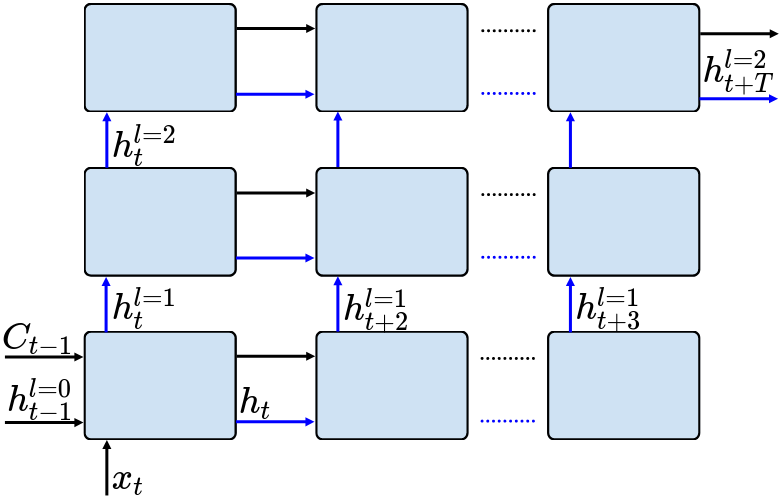
\includegraphics[width=0.99\textwidth]{figures/lstm}
  \caption{Long-short-term-memory (LSTM)}
  \label{fig:sub1}
\end{subfigure}%
\begin{subfigure}{.5\textwidth}
  \centering
  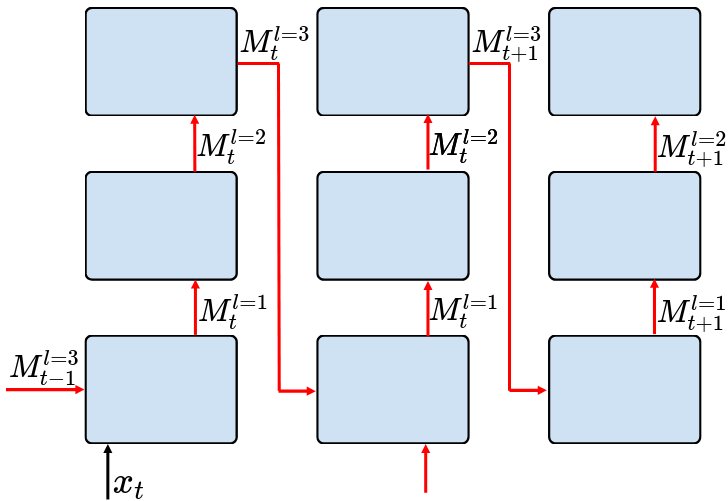
\includegraphics[width=0.88\textwidth]{figures/stlstm}
  \caption{Spatio-temporal LSTM (ST-LSTM)}
  \label{fig:sub2}
\end{subfigure}
\caption{Comparison of the computational flow within a stacked LSTM and a stacked ST-LSTM. The red arrows mark the additional computations of the $M$-state}
\label{fig:stlstmcell}
\end{figure}


%\subsubsection{Convolutional LSTM}\label{cap:CLSTM}
%At least since the performance of convolutional neural networks (CNNs) in the ImageNet competition \cite{ILSVRC15} for image classification, it is empirically proven that CNNs are more effective in certain computer vision tasks, than fully connected neural networks.
%In the field of sequential learning, computer vision tasks are also formulated, such as video-classification or video-frame interpolation. The second experiment is also a type of vision task. However, LSTMs as implemented in the equation from \ref{eq:lstm} can be regarded as recurrent extension of a fully connected neural network, which is not as efficient in processing spatial correlations as a CNN. 

%A LSTM with convolutional structure addresses this problem. It is better performing in certain tasks which include spatio-temporal data, as proven for example by Wu et al. for future video synthesis \cite{wu_future_2020}. This concept is used in the second experiment of this work, which also deals with the processing of spatio-temporal data.

%The equations, which build a convolutional LSTM, are shown below:

%\begin{align}
%    g_t&=\tanh\left(\textbf{W}'_{cx}*x_t + \textbf{W}'_{ch}* h_{t-1} + b_g\right), \notag\\
%    f_t&=\sigma\left(\textbf{W}'_{fx}* x_t + \textbf{W}'_{fh}* h_{t-1} + b_f\right), \notag\\
%    i_t&=\sigma\left(\textbf{W}'_{ix}* x_t + \textbf{W}'_{ih}* h_{t-1} + b_i\right), \notag\\
%    o_t&=\sigma\left(\textbf{W}'_{ox}*x_t + \textbf{W}'_{oh}* h_{t-1} + b_o\right), \notag\\
%    C_t&=f_t\circ C_{t-1}+i_t\circ g_t, \notag\\
%    h_t&=o_t\circ\tanh(C_t).\notag\\
%\end{align}

%As introduced in chapter \ref{cap:kernel_convolution}, the symbol * denotes a discrete convolution while the operators $\textbf{W}'$ are convolutional kernel. The only difference from a regular LSTM is that the linear operators are replaced by convolutional operators. This version of a LSTM can handle a sequence of spatial data without flattening them to a vector.

%\subsubsection{Spatio-temporal LSTM} \label{cap:STLSTM}
%The performance of a LSTM network depends on how good it is capable of memorizing relevant structures. 

%As introduced before, a convolutional LSTM is taking into account advantages of convolutions to compute spatial correlation more efficiently. However, in a stacked convolutional LSTM, spatial correlations and temporal dynamics are not equally processed \cite{prednet}, however, these two aspects might be equally important and should be considered equally significant in a machine learning model for spatio-temporal data. To address this problem, Y. Wang et al. introduce in their paper \textit{PredRNN: Recurrent Neural Networks for Predictive Learning using Spatio-temporal LSTMs} \cite{prednet} a variation of the LSTM and its integration into a stacked recurrent neural network. They do not define how to measure the equality in processing the two aspects (spatial correlations and temporal dynamics) but they formulate it as follows:


To address this problem they invented a variation of a LSTM, the spatio-temporal LSTM (ST-LSTM), which is defined by:

\begin{align}\label{eq:stlstm}
    g_t&=\tanh\left(\textbf{W}'_{cx}*x_t + \textbf{W}'_{ch}* h_{t-1} + b_g\right),\notag\\
    i_t&=\sigma\left(\textbf{W}'_{ix}* x_t + \textbf{W}'_{ih}* h_{t-1} + b_i\right),\notag\\
    f_t&=\sigma\left(\textbf{W}'_{fx}* x_t + \textbf{W}'_{fh}* h_{t-1} + b_f\right),\notag \\
    C_t&=f_t\circ C_{t-1}+i_t\circ g_t,\notag\\
    g'_t&=\tanh\left(\textbf{W}''_{cx}*x_t + \textbf{W}'_{cm}* M^{l-1}_{t} + b'_g\right),\notag\\
    i'_t&=\sigma\left(\textbf{W}''_{ix}* x_t + \textbf{W}'_{im}* M^{l-1}_{t} + b'_i\right),\notag\\
    f'_t&=\sigma\left(\textbf{W}''_{fx}* x_t + \textbf{W}'_{fm}* M^{l-1}_{t} + b'_f\right),\notag\\
    M^{l}_t&=f'_t\circ M^{l-1}_t+i'_t\circ g'_t\notag\\
    o_t&=\sigma\left(\textbf{W}'_{ox}*x_t + \textbf{W}'_{oh}*h_{t-1} + \textbf{W}_{om}*M_t^l + b_o\right),\notag\\
    h_t&=o_t\circ\tanh(\textbf{W}_{1\times 1}*\left[C_t^l,M_t^l\right]).\notag\\
\end{align}

The difference to a normal LSTM is that here the states ($C$, $h$ and additionally $M$) are not exclusively evolved in time and then transmitted to the next layer. First, the cell state $M$ evolves through the layers of the stacked ST-LSTM, and is then passed to the input of the next time step at the bottom of the network. The idea of this LSTM adaptation is visualized in at \textbf{(b)} of figure \ref{fig:stlstmcell}. The first figure is a visualization of the computations in a enfolded LSTM network with three stacked layers, while the second one shows an unfolded ST-LSTM. The red line is the computational flow of the cell state $M$ in the computational graph.

%\begin{figure}[ht]
%    \center
%    \includegraphics[width=0.99\textwidth]{figures/stlstm_cell.png}
%	\caption{Visualizations of the computations in a spatio-temporal LSTM cell. The orange parts show the additional calculation steps to a LSTM cell \cite{prednet}.}
%	\label{fig:stlstmcell}
%\end{figure}

%\begin{figure}[ht]
%    \center
%    \includegraphics[width=0.99\textwidth]{figures/unfolded_stlstm.png}
%	\caption{Visualizations of a stacked spatio-temporal LSTM, unfolded through time. The orange arrow marks the computational flow through the layers of the network and time steps of the input sequence \cite{prednet}.}
%	\label{fig:unfolded_stlstm}
%\end{figure}

%\begin{figure}[ht]
%center
%    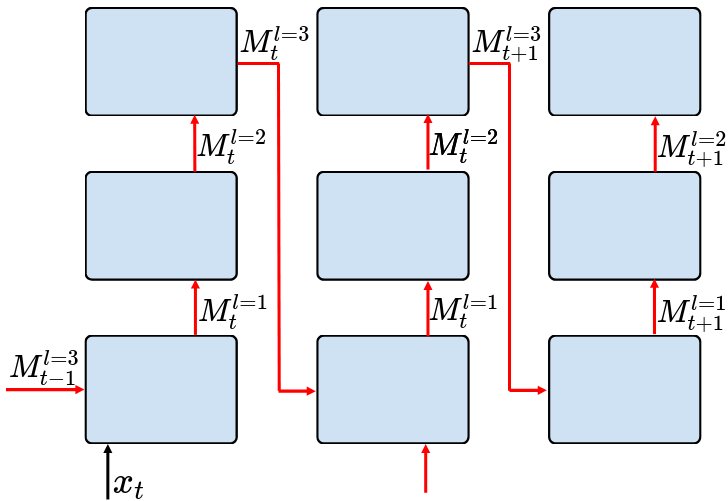
\includegraphics[width=0.99\textwidth]{figures/stlstm}
%	\caption{Two visualizations of a Spatio-temporal LSTM, where the left figure shows graphically the computations inside the ST-LSTM-cell, while the right one visualizes the unfolded cell through time. The orange arrow marks the computational flow through the layers of the network and time-steps of the input-sequence \cite{prednet}.}
%	\label{fig:seq2seq}
%\end{figure}

%LSTMs are the favored implementation of recurrent neural networks. It is a standard to overcome general problems like vanishing gradient and learning long-term dependencies. Additionally, convolutional LSTMs or spatio-temporal LSTMs are designed to specifically face problems which occur in deep LSTMs where spatial correlation and temporal dynamics are not equally processed.

Although the special kind of LSTM have been mentioned so far, it is not yet clear how exactly this iterative process can be used to face a (seq2seq) problem such as it is posed in this numerical experiment.

\subsubsection{Seq2Seq-models} \label{cap:seq2seq}
%introduction, and problems to face
A common design for a LSTM-neural network to address a seq2seq problem is an encoder-decoder model. It consists of two LSTMs, one for encoding the sequence to a \textit{thought vector} of fixed dimension, and the other for generating an output sequence with varying length from the thought vector. The thought vector consists of the respective states, which are the hidden state $h$, and cell state $C$, with an additional state $M$, in case of a ST-LSTM. In the example of an encoder-decoder network (figure \ref{fig:encoder_decoder}), each time step of the input sequence is processed by an encoder independently, such as the output sequence is processed by the decoder (purple parts in the figure). The input sequence of the decoder LSTM (blue parts at the right side of the graphic) is built by a sequence of the same $h$-value from the thought vector, for every step. Therefore, every iteration in the LSTM takes into account the same representation of the input sequence while evolving another $h$- and $C$-value (and probably additionally $M$) with every iteration.

\begin{figure}[ht]
    \center
    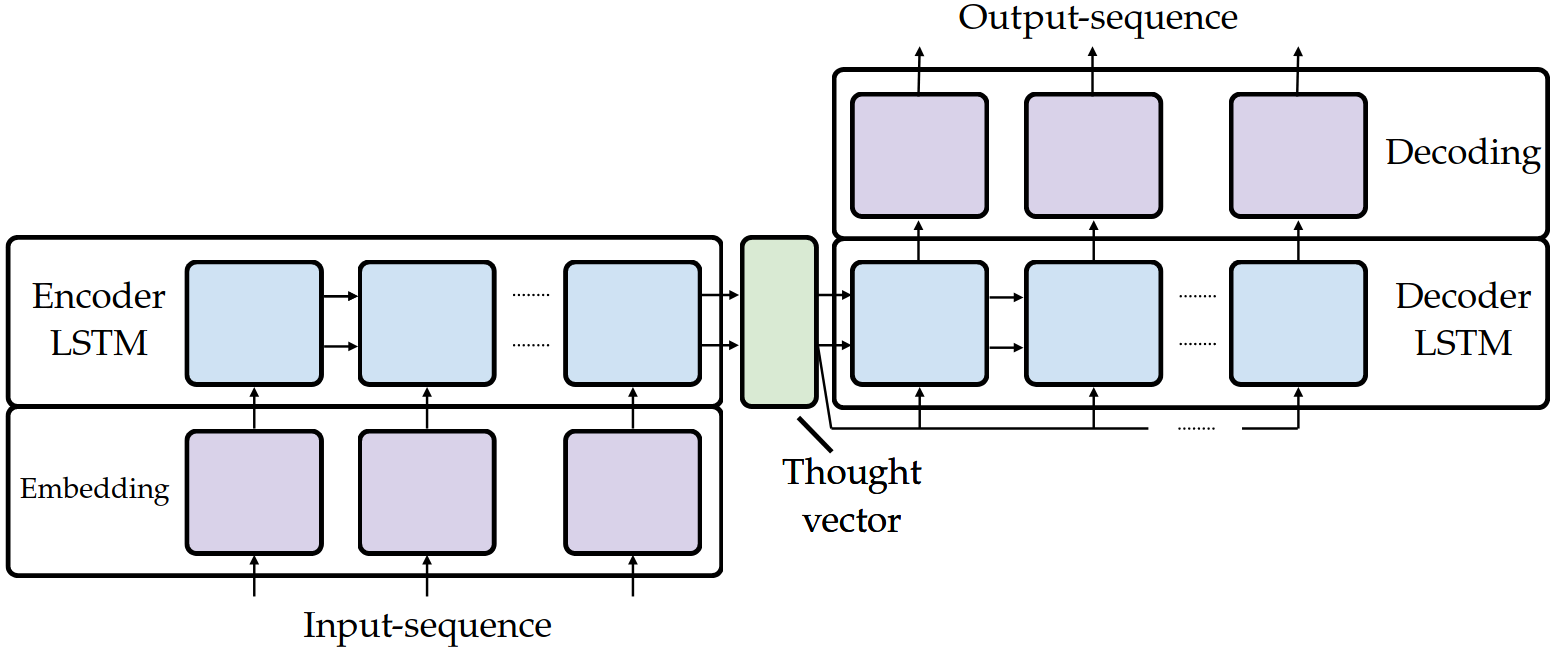
\includegraphics[width=0.70\textwidth]{figures/encoder_decoder_schematic}
	\caption{Schematic sequence-to-sequence model (seq2seq) with an encoder-decoder structure.}
	\label{fig:encoder_decoder}
\end{figure}

%Within the second experiment (chapter 4), this kind of neural network is used as well. It consists of convolutional neural networks for embedding and decoding and is combined with stacked convolutional LSTMs (and ST-LSTM as well) for seq2seq-processing.
\section{Results}

To quantify the reconstruction of the neural networks, we calculate the point wise absolute error between the predicted values of $u$ of the voxels and their true values. The errors are then averaged layer wise, that one gets a mean absolute error per predicted layer. In section \ref{sec:T} we show the results of several trained neural networks of the same type, where the input sequence length is varied. It is tested with the two regimes (A and B), where A has periodic dynamic and B show chaotic behaviour. The best model, considering our error measurement from this experiment, is then taken for further examination in the section afterwords, where the reconstruction target changes. Furthermore, its results are compared to another neural network, which is based on convolutions and a conditional random field.

\subsection{}\label{sec:T}

Figures:
\begin{itemize}
    \item Full 3d cube with prediction
    \item Gridplot, different T
    \item MAE comparison with different Depths
    \item Comparison with Sebastian's model
\end{itemize}

% Up to three levels of \textbf{subheading} are permitted. Subheadings should not be numbered.
%- Machine learning results: learning time, etc.
%- how deep can we look? (still needed: spatial correlation)

%\subsection{Data}
%-> Copy equations from master thesis
%-> 3d plots of dynamics (fig 4.2)
%-> further characterization of data?
%-> characteristic numbers (time, spatial, velocity)

%-> two parameter sets of barkley model
%-> Parameter sets used
%-> N initial conditions for both, example snapshots after transient
%-> some characterisation (periodic, see figure figPeriodic, chaotic as can be estimated from figure figchaotic)

%\subsection*{Machine Learning}

%(Machine learning) experiment used. Parameter, model, references, explanation via a figure



%\subsection*{Subsection}

%Example text under a subsection. Bulleted lists may be used where appropriate, e.g.


%\subsubsection*{Third-level section}
%Topical subheadings are allowed.
\section*{Discussion}

The Discussion should be succinct and must not contain subheadings.

\bibliography{sample}

\noindent LaTeX formats citations and references automatically using the bibliography records in your .bib file, which you can edit via the project menu. Use the cite command for an inline citation, e.g.  \cite{Hao:gidmaps:2014}.

For data citations of datasets uploaded to e.g. \emph{figshare}, please use the \verb|howpublished| option in the bib entry to specify the platform and the link, as in the \verb|Hao:gidmaps:2014| example in the sample bibliography file.

\section*{Acknowledgements (not Xsub = Xcompulsory)}

Acknowledgements should be brief, and should not include thanks to anonymous referees and editors, or effusive comments. Grant or contribution numbers may be acknowledged.

\section*{Author contributions statement}
Must include all authors, identified by initials, for example:
A.A. conceived the experiment(s),  A.A. and B.A. conducted the experiment(s), C.A. and D.A. analysed the results.  All authors reviewed the manuscript. 

\section*{Additional information}

To include, in this order: \textbf{Accession codes} (where applicable); \textbf{Competing interests} (mandatory statement). 

The corresponding author is responsible for submitting a \href{http://www.nature.com/srep/policies/index.html#competing}{competing interests statement} on behalf of all authors of the paper. This statement must be included in the submitted article file.

% \begin{figure}[ht]
% \centering
% \includegraphics[width=\linewidth]{stream}
% \caption{Legend (350 words max). Example legend text.}
% \label{fig:stream}
% \end{figure}

% \begin{table}[ht]
% \centerin
% \begin{tabular}{|l|l|l|}
% \hline
% Condition & n & p \\
% \hline
% A & 5 & 0.1 \\
% \hline
% B & 10 & 0.01 \\
% \hline
% \end{tabular}
% \caption{\label{tab:example}Legend (350 words max). Example legend text.}
% \end{table}

% Figures and tables can be referenced in LaTeX using the ref command, e.g. Figure \ref{fig:stream} and Table \ref{tab:example}.

\end{document}